\documentclass[11pt]{article}

\usepackage[utf8]{inputenc}
\usepackage{fancyhdr}
\usepackage{hyperref}
\usepackage{graphicx}
\usepackage{amsmath}
\usepackage{amssymb}
\usepackage{natbib}

\graphicspath{ {images/} }
 
\pagestyle{fancy}
\fancyhf{}
\lhead{University of the Witwatersrand}
\rfoot{School of Computer Science and Applied Mathematics}
\pagenumbering{roman}
\fancyfoot[R]{\thepage}
\renewcommand{\headrulewidth}{0pt} % to remove line on header
\renewcommand{\footrulewidth}{0pt} % to remove line on footer

\begin{document}
\begin{page}
\thispagestyle{empty}

\newcommand{\HRule}{\rule{\linewidth}{0.3mm}} % Defines a new command for the horizontal lines, change thickness here
\renewcommand\section{\@startsection{section}{1}{\z@}%
                                  {-3.5ex \@plus -1ex \@minus -.2ex}%
                                  {2.3ex \@plus.2ex}%
                                  {\normalfont\large\bfseries}}
\setlength{\parindent}{0pt}

\center % Center everything on the page
 
%----------------------------------------------------------------------------------------
% HEADING SECTIONS
%----------------------------------------------------------------------------------------

\textsc{\LARGE University of the Witwatersrand}\\[1.5cm] % Name of your university/college
\textsc{\Large School of Computer Science and Applied Mathematics}\\[0.5cm] % Major heading such as course name

%----------------------------------------------------------------------------------------
% TITLE SECTION
%----------------------------------------------------------------------------------------

\HRule \\[0.4cm]
{ \huge \bfseries COMS3008: Parallel Computing Lab Assignment 3}\\[0.4cm] % Title of your document \\
  \large 25 July 2016
\HRule \\[1.5cm]
 
%----------------------------------------------------------------------------------------
% AUTHOR SECTION
%----------------------------------------------------------------------------------------
\begin{minipage}{1\textwidth}
  \Large \emph By Chalom, J. (711985)\\
\end{minipage}


\vfill % Fill the rest of the page with whitespace

\end{page}

\begin{page}
\rfoot{School of Computer Science and Applied Mathematics}
\clearpage
\setcounter{page}{1}
\pagenumbering{arabic}

\section{General Assumptions and Methodology}
All drawn diagrams were drawn using \url{http://draw.io/}, and all results from empirical analysis, were statistically analysed by the data processing program used in lab 1. Those averaged results were then plotted using Microsoft Excel.\\

\noindent The system used for empirical analysis, had an i3 Ivy-bridge CPU, with four processing units and 8GB of RAM.\\

\noindent \large \chapter{\textbf{Glossary Of Terms:}}\\\\
\noindent \textbf{\textit{Trapezoid}} - is defined as the British definition (Trapezium) as a quadrilateral with no sides parallel \\
\noindent \textbf{\textit{IBT}} - is an acronym for integration by parts.\\
\noindent \textbf{\textit{STR}} - is an acronym for Simpson's Trapezoidal Rule.\\
\noindent \textbf{\textit{CTR}} - is an acronym for Composite Trapezoidal Rule.\\

\section{Analytical Solution of Given Integral}
\noindent Let $f(x) = \int_{0}^{20} xe^{-x} dx$\\
\\
\noindent By IBT let $\int fdg = fg - \int gdf$, \\
where $f = x$, $dg = e^{-x} dx$, $df = dx$ and $g = -e^{-x}$.\\

\begin{equation} 
\begin{aligned}
    \therefore{} \int xe^{-x} dx = -e^{-x} + \int e^{-x} dx\\ 
\end{aligned}
\end{equation}
\\
\noindent Let $u = -x$ and $dy = -dx$

\begin{equation}
\begin{aligned}
    \therefore{} -e^{-x} + \int e^{-x} dx &= -e^{-x}x - \int e^{u} du\\
    & = -e^{u} - e^{-x}x + c\\
    & = -e^{-x} - e^{-x} + c 
\end{aligned}
\end{equation}
\\

\begin{equation}
\begin{aligned}
    \therefore{} \int_{0}^{20} xe^{-x} dx &= \left[-e^{-x} - e^{-x} + c\right]_{0}^{20} \\
    & = -e^{-20}(20) - e^{-20} + e^{0}(0) + e^{0}\\
    & = 1 + \epsilon{}\\
    & \simeq{} 1,00
\end{aligned}
\end{equation}

Note: $\epsilon{} \simeq{} -4,329422607 x 10^{-8}$
\\

\section{Parallel Trapezoidal Integration}
\noindent \chapter{The Trapezium:}\\
\noindent Let $a$ be the top section of a trapezoid (Fig 1), $b$ be the base of a trapezoid (Fig 1) and $h$ be the greatest height between $a$ and $b$.

\begin{figure}[ht]
\centering
     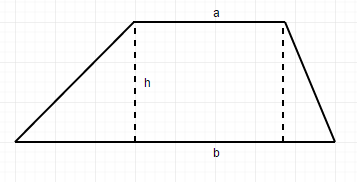
\includegraphics[width=1.00\textwidth]{trapezium}\\
     Fig 1. An example trapezium
\end{figure}

\noindent The area of a trapezoid is defined as: $A = \frac{a+b}{2}h$\\
\\

\break

\noindent \chapter{Derivation of the Trapezoidal Rule (STR):}\\
\noindent Let $P_n$ be a polynomial function of n terms.\\

\begin{equation}
\begin{aligned}
    \int_{a}^{b} P_n(x) dx &\simeq{} \int_{a}^{b} f[a]dx + \int_{a}^{b} f[a,b](x-a)dx\\
    &\simeq{} (b-a)f(x) + (\frac{f(b)-f(a)}{(b-a)}).\frac{1}{2}(x-a)^{2}]_{a}^{b}\\
    &\simeq{} (b-a)f(a) + (\frac{f(b)-f(a)}{(b-a)}).\frac{1}{2}(b-a)^{2}\\
    &\simeq{} \frac{b-a}{2}(f(a)+f(b))
\end{aligned}
\end{equation}

\begin{equation}
\begin{aligned}
    Error = \frac{-(b-a)^{3}}{12}f^{''}(\phi)
\end{aligned}
\end{equation} 
\\

\noindent \chapter{Derivation of the Composite Trapezoidal Rule (CTR):}\\
\noindent For sub-intervals: $a = x_0 < x_1 < ... < x_n = b$
\\

\begin{figure}[ht]
\centering
     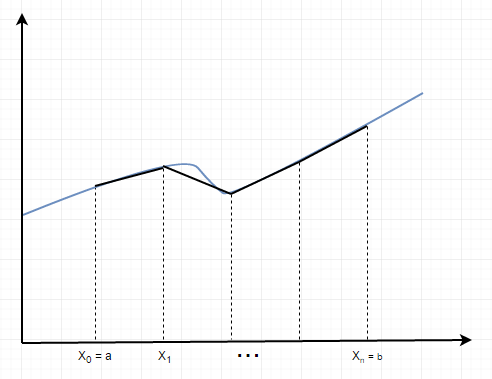
\includegraphics[width=0.80\textwidth]{approx_graph}\\
     Fig 2. Approximation of a polynomial
\end{figure}
\\
\begin{equation}
\begin{aligned}
    n &= \frac{b-a}{m}\\
    & = \Delta{x}\\
    & = (x_1 - x_0)
\end{aligned}
\end{equation}
Note: $\Delta{x}$ is fixed.
\\
\begin{equation}
\begin{aligned}
    \int_a^b f(x) dx &= \int_{a=x_0}^{x_1} f(x) + \int_{x_1}^{x_2} f(x) + ... + \int_{x_{n-1}}^{x_n=b} f(x)\\
    &\simeq{} (\frac{x_1 - x_0}{2})[f(x_0) + f(x_1)] + ... + (\frac{x_m - x_{m-1}}{2})[f(x_{m-1}) + f(x_m)]\\
    &\simeq{} \frac{n}{2}[f_0 + 2f_1 + 2f_2 + ... + 2f_{m-1} + f_m]
\end{aligned}
\end{equation}
\\

\begin{equation}
\begin{aligned}
    Error_C_T_R = \frac{(b-a)^3}{12m^2}$ $f^{0}(\phi)$, $\phi \in [a,b]
\end{aligned}
\end{equation}
\\\\


\noindent \chapter{Implementation Results:}\\

\noindent \chapter{Implementation Analysis:}\\

\section{Parallel Monte Carlo Integration}
\noindent \chapter{:} 

\end{page}


\end{document}
